

\section{Data preparation}

The COMPAS dataset used in this study is publicly available through ProPublica's GitHub repository. This repository contains the dataset and other assets used by ProPublica to investigate the biases present in the COMPAS risk assessment tool.

The file chosen for this analysis is \textbf{\texttt{compas-scores-two-years.csv}}, as it provides the cleanest and most relevant data for general recidivism prediction. This CSV file contains the key data required for our study, including several attributes related to demographics, criminal history, COMPAS risk scores, and the two-year recidivism outcomes that are important for exploring the predictive capabilities and the ethical implications of machine learning models in the context of recidivism prediction. 

The dataset includes important information about individuals. Following an initial analysis, a list of the key fields in the dataset is below.

\begin{itemize}
	
	\item Personal Information, includes attributes such as \textbf{\texttt{age}}, \textbf{\texttt{race}}, \textbf{\texttt{age\_category}}, etc.
	
	\item Case and Event-Related Details are the fields prefixed with \textbf{\texttt{c\_}} that provide a timeline and details of a person's interactions with the criminal justice system.
	
	\item Violence Risk Assessment are the fields prefixed with \textbf{\texttt{v\_}} and are associated with the violence risk assessment in COMPAS. This dimension predicts violent recidivism risk.
	
	\item Case-Level Details for Violent Recidivism are the fields prefixed with \textbf{\texttt{vr\_}}. These fields provide additional details specific to violent recidivism events.
	
	\item Juvenile Criminal Record are the fields prefixed with \textbf{\texttt{juv\_}}. These fields capture information about an individual's juvenile criminal record, which is a key predictor of future adult criminal behaviour.
	
	\item Previous Charges and Severity can be deduced from fields such as \textbf{\texttt{priors\_count}} and \textbf{\texttt{juv\_}} fields.
	
	\item Additional fields, including \textbf{\texttt{r\_charge\_}}, \textbf{\texttt{r\_offense\_}}, \textbf{\texttt{vr\_}} fields, \textbf{\texttt{c\_charge\_degree}}, and \textbf{\texttt{c\_charge\_desc}}, provide a broader perspective on criminal history and severity.
	
	
	\item Two-Year Recidivism, or the \textbf{\texttt{two\_year\_recid}} field in the COMPAS dataset, indicates whether an individual reoffended (recidivated) within two years of their initial assessment or release. This field is critical for evaluating the predictive accuracy of the COMPAS risk assessment tool.
	
	\item Decile Score is a standardized risk score in the COMPAS dataset. It categorizes an individual's likelihood of recidivism into ten equal groups (deciles) where 1 is the lowest risk, and 10 is the highest risk. Each decile represents approximately 10\% of the sample when applied to a norm group.
	
\end{itemize}

%Suppose that we observe the following data:

%\begin{table}[!ht]
%	\centering
%	\begin{tabular}{|l|l|}
%		\hline
%		Field & Value \\ \hline
%		\textbf{\texttt{priors\_count}} & 5 \\ \hline
%		\textbf{\texttt{juv\_felony\_count}} & 2 \\ \hline
%		\textbf{\texttt{juv\_misdemeanor\_count}} & 3 \\ \hline
%		\textbf{\texttt{r\_charge\_degree}} & Felony \\ \hline
%	\end{tabular}
%\end{table}

%We can interpret this as an individual who has five total prior charges, including:

%\begin{itemize}
%	\item 2 juvenile felonies
%	\item 3 juvenile misdemeanours
%	\item The severity of previous charges includes felonies (\textbf{\texttt{r\_charge\_degree}}).
%\end{itemize}


\subsection{Preparing the data for further analysis and training}

Before we can perform any analysis or apply machine learning techniques, it is important to pre-process and prepare the dataset so that we can handle missing values, encode categorical features, and split the data into training, testing, and validation sets. This step will produce a clean dataset for building accurate and unbiased models. The following steps outline the procedures to prepare the dataset for further analysis and training.


\subsection{Initial look at data and missing values handling}

The dataset has 7214 instances over 53 columns. The target of the dataset is \textbf{\texttt{decile\_score}}, but the dataset also contains information about whether or not the person recidivised, most notably through the label \textbf{\texttt{two\_year\_recid}}. 

The first step in data preparation is removing the features irrelevant to this exercise or with over 50\% missing records. We removed all the COMPAS-administrative labels and additional recidivism information apart from \textbf{\texttt{two\_year\_recid}}, narrowing the dataset to 17 fields.

The difference between \textbf{\texttt{c\_jail\_in}} and \textbf{\texttt{c\_jail\_out}} was calculated into a new field, \textbf{\texttt{days\_in\_jail}} and the difference between \textbf{\texttt{in\_custody}} and \textbf{\texttt{out\_custody}}, in a new field, \textbf{\texttt{days\_in\_custody}}. We subsequently removed the features containing date information from the dataset, together with \textbf{\texttt{days\_in\_custody}}, as it contained no information. At this stage, the dataset contains thirteen features: eight numerical, four categorical, and one descriptive. It also contains two labels, decile\_score, which we will treat as the leading label in this exercise and \textbf{\texttt{two\_year\_recid}}, which we are keeping to compare the prediction power of our models to the original one.


\subsection{Imputation of missing data}

While examining the resultant dataset, we noticed that \textbf{\texttt{days\_b\_screening\_arrest}} has  6907 values that are not null. Whilst it is possible to eliminate the rows that contain the null values at this stage, we replaced the missing values using a KNN imputation technique by grouping the numeric values of this dataset so that we can calculate the missing values. We checked this process by plotting the distribution of \textbf{\texttt{days\_b\_screening\_arrest}} before and after imputation to see if any variations occurred.

\begin{figure}[h!]
	\centering
	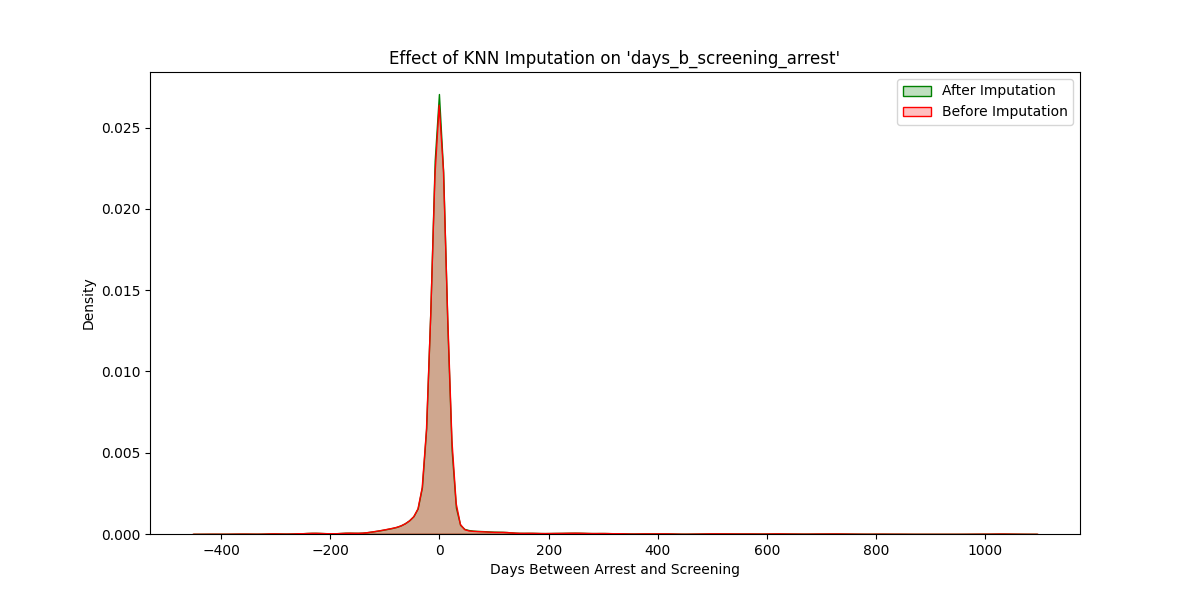
\includegraphics[width=0.9\linewidth]{img/imputation}
	\caption[Distribution \textbf{\texttt{days\_b\_screening\_arrest}} of before and after KNN imputation]{}
	\label{fig:imputation}
\end{figure}

At this stage, the dataset contains four categorical features that need encoding for machine learning algorithms. This section will focus on converting them into a numerical format using two encoding techniques. The categorical features and their values are listed below:

\begin{table}[!ht]
	\centering
	\begin{tabular}{|l|l|l|}
		\hline
		Feature & Description & Unique Values \\ \hline\hline
		\textbf{\texttt{sex}} & Gender of the individual & \shortstack{Male\\Female} \\ \hline
		\textbf{\texttt{race}} & Race of the individual & \shortstack[l]{African-American\\Caucasian\\Hispanic\\Asian\\Native American\\Other} \\ \hline
		\textbf{\texttt{age\_cat}} & Age category & \shortstack[l]{Less than 25\\25 - 45\\Greater than 45} \\ \hline
		\textbf{\texttt{c\_charge\_degree}} & Degree of the criminal charge & \shortstack[l]{F (Felony)\\M (Misdemeanor)} \\ \hline
	\end{tabular}
\end{table}

The following transformations are applied:

\begin{itemize}[]
	\item One-Hot Encoding on \textbf{\texttt{sex}}, \textbf{\texttt{race}}, and \textbf{\texttt{c\_charge\_degree}}, transforming them into binary columns.
	\item Ordinal Encoding on \textbf{\texttt{age\_cat}}. This encoding technique was preferred over one-hot in this case as it preserves order,thus respecting the inherent ranking of the category.
\end{itemize}

The original categorical columns were retained in the dataset for future use in the analysis steps. 

\subsection{Splitting the data into train, test and dev}

A stratified shuffle split technique is preferred to create the train, test, and dev datasets whilst ensuring that the splits are proportional by \textbf{\texttt{race}}. In the first split, 80\% Train and 20\% Test are created, whilst in the Second split, The 20\% Test is further divided into 10\% Test and 10\% Dev.


\section{Data exploration and visualisation}

This section will examine the dataset in more detail to understand the patterns, distributions, and relationships. In this exercise, we will use more of the visual tools available through several Python libraries to identify potential biases, explore correlations between variables, and uncover insights that may influence the outcomes of predictive models. 

\subsection {Demographic analysis}

We begin this analysis by segmenting the dataset based by race and gender.


% First image
\begin{figure}
	\centering
	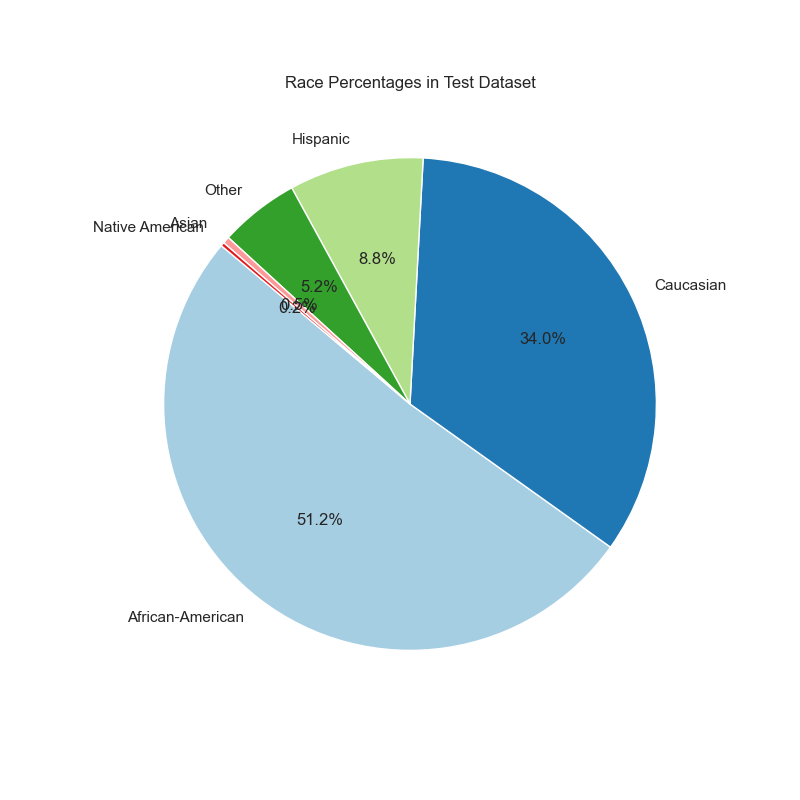
\includegraphics[width=0.7\linewidth]{img/race_percentages_pie.png}
	\caption{Caption for the first image}
	\label{fig:image1}
\end{figure}
\hfill
% Second image
\begin{figure}
	\centering
	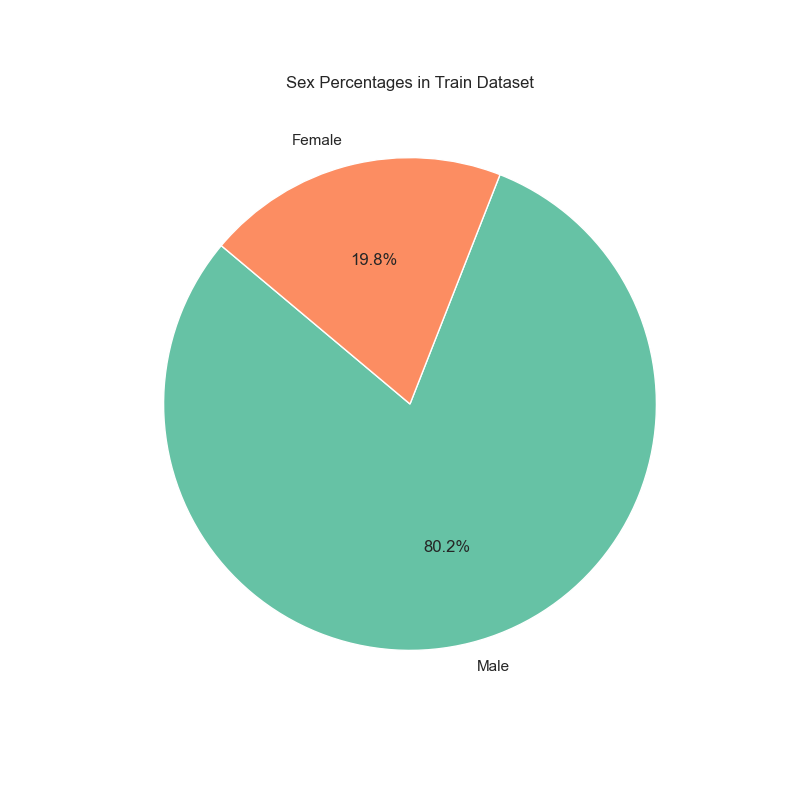
\includegraphics[width=0.7\linewidth]{img/sex_percentages_pie.png}
	\caption{Caption for the second image}
	\label{fig:image2}
\end{figure}


By examining the racial composition of the dataset, we observe the following:

\begin{itemize}
	\item Over half of the test dataset is composed of African-American individuals, suggesting that the dataset may be imbalanced, with a disproportionate representation of one racial group.
	\item Asians and Native Americans each makeup only 0.2\% of the dataset; this underrepresentation might raise some concerns as it may lead to challenges in statistical analysis or machine learning models. Such concerns include the lack of reliability or significance for these groups due to insufficient data.
\end{itemize}

Figure \ref{fig:race-sex-breakdown} also shows our dataset's male/female split, with females comprising only 19.8\%. It is, therefore, evident that the female group is underrepresented, which can lead to biased models as models may overfit male patterns and underperform on females and misleading conclusions as insights derived might generalise poorly for the female subgroup.


\subsection{Age distribution analysis}


We used a boxplot to illustrate the age patterns across racial groups, helping to identify central values, spread, and any anomalies.

\begin{figure}[H]
	\centering
	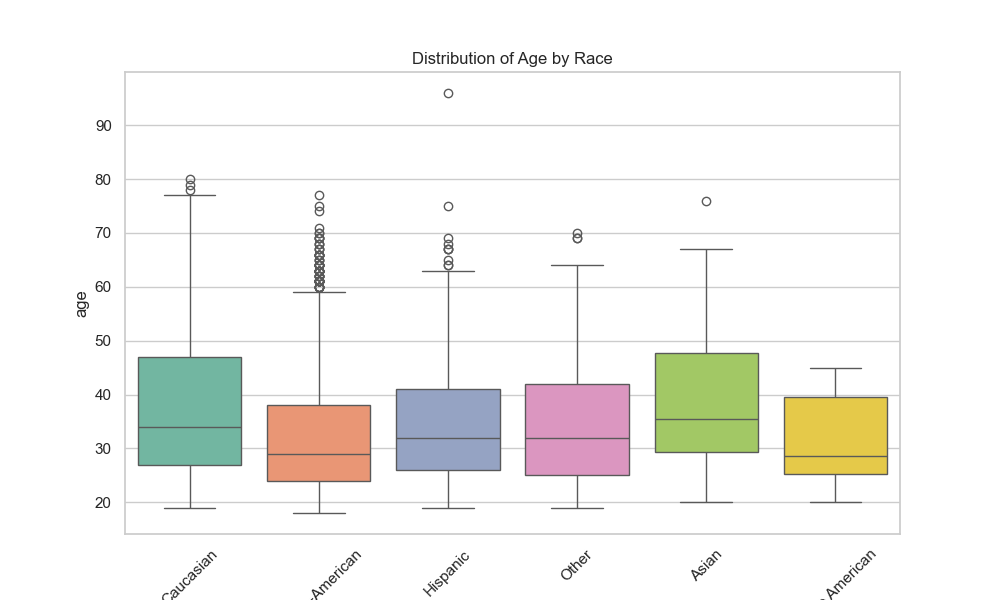
\includegraphics[width=0.9	\linewidth]{img/age_by_race_boxplot}
	\caption{}
	\label{fig:age-by-race-boxplot}
\end{figure}



\begin{table}[H]
	\centering
	\begin{tabular}{|l|l|p{4cm}|}
		\hline
		Race & Median Age & Distribution Description \\ \hline \hline
		African-American & $\approx$30 years & Concentrated in the 20–40 range, with a relatively narrow spread. We notice outliers above 60 years,  indicating fewer older individuals. \\ \hline
		Caucasian & $\approx$40 years & Broader age range, from 20 to 70+ years. We notice more older individuals (upper outliers), making this group appear older on average. \\ \hline
		Hispanic & $\approx$30–35 years & Moderately broad spread, with most individuals between 20 and 50 years. \\ \hline
		Asian & $\approx$30 years & Narrow distribution, concentrated between 25 and 40 years. No outliers. \\ \hline
		Native American & $\approx$33 years & Very tight distribution, with all ages clustered closely around the median (little variability). It is important to note that this group accounts for a tiny portion of the population. \\ \hline
		Other & $\approx$35–40 years & Similar to Caucasians but with slightly fewer older individuals. The IQR shows a widespread. \\ \hline
	\end{tabular}
\end{table}



\subsection{Analysing distributions}


Next, we plotted the distributions of all the features in our dataset; this is depicted in Figure \ref{fig:distribution-plots} . From these histograms, we notice 
\begin{itemize}
	\item The age distribution shows a right-skewed pattern, with most individuals falling in the younger age ranges (20–40 years).
	
	\item There is a significant over-representation of certain racial groups, particularly African Americans, which could indicate potential biases in the dataset's sampling.
	
	\item Most individuals have zero juvenile felony counts, zero juvenile misdemeanour counts, and no recorded "other" juvenile offences, with each distribution rapidly declining for higher counts.
	
	\item A large proportion of individuals have a low number of prior offences, but there is a long tail indicating some individuals have a significant number of priors.
	
	\item Most individuals have relatively short jail durations, with a few experiencing significantly longer durations.
	
	\item The distribution of days between screening and arrest is clustered around zero, with few extreme outliers on both ends.
	
	\item The decile scores appear relatively evenly distributed, but slight patterns suggest clustering at specific score levels (e.g., lower decile scores are slightly more frequent).
	
	\item Two-year recidivism plot shows a near-equal distribution, indicating a balanced dataset for recidivism outcomes.
\end{itemize}


\begin{figure}[H]
	\centering
	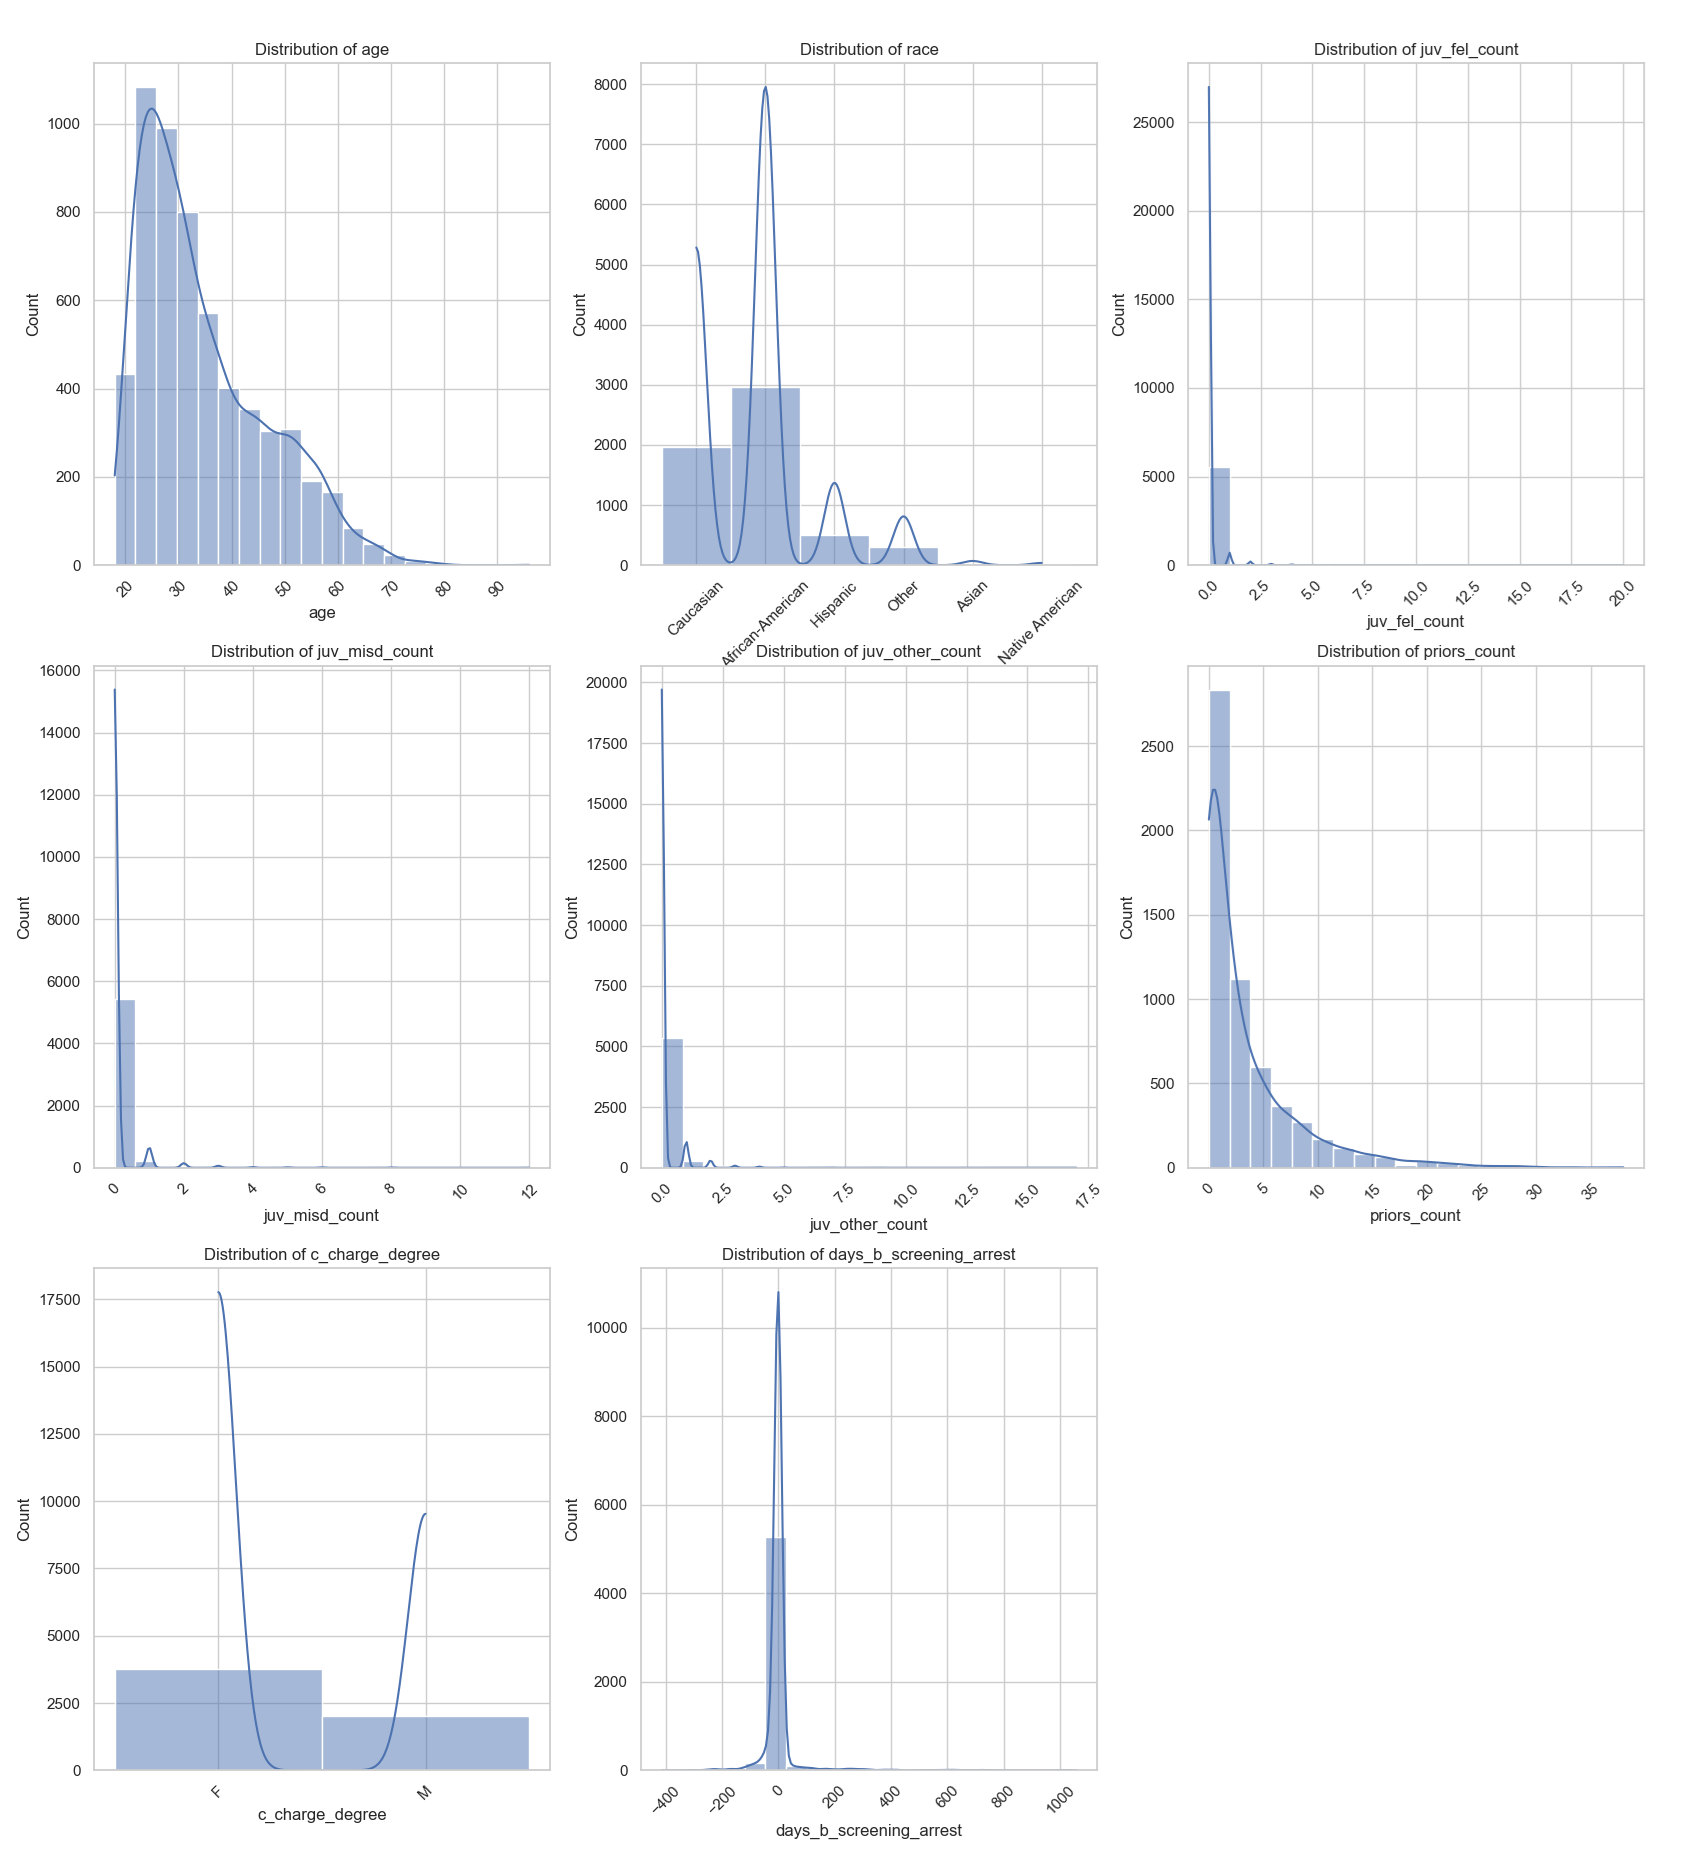
\includegraphics[width=0.9\linewidth]{img/distribution-plots}
	\caption{}
	\label{fig:distribution-plots}
\end{figure}


\subsection{Correlation analysis}

The correlation matrix heatmap shown in Figure \ref{fig:correlationmatrixheatmap} was created to gather more insights and pinpoint the areas of high correlation. This plot raises a number of interesting observations, namely:

\begin{figure}[!h]
	\centering
	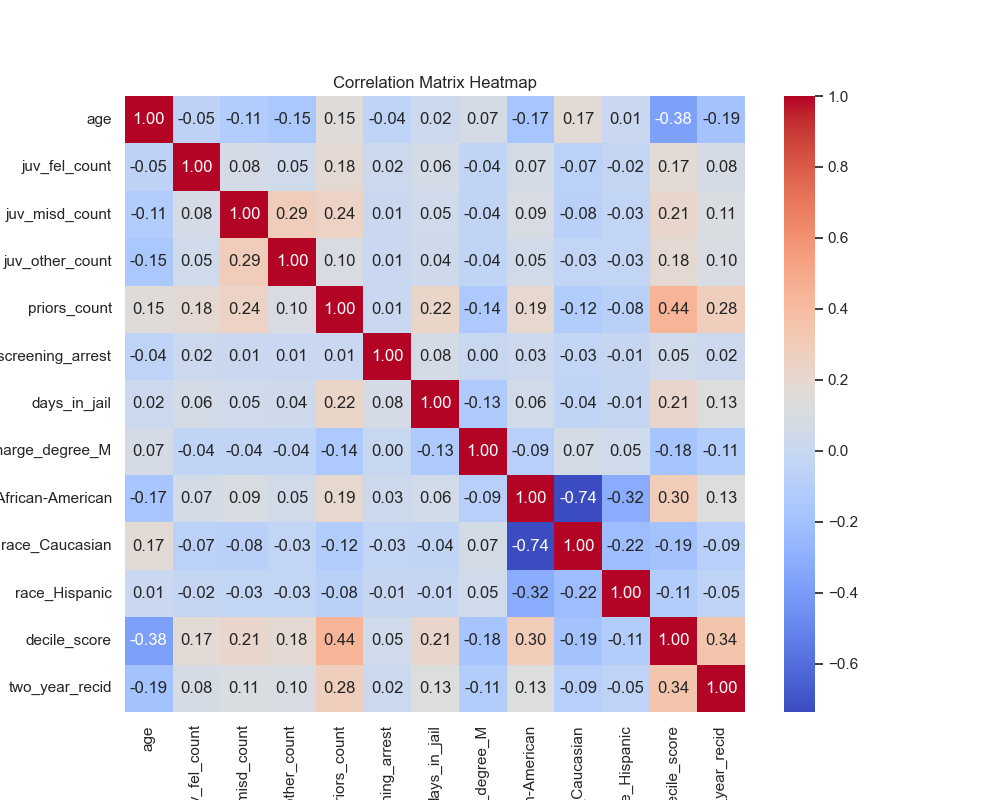
\includegraphics[width=0.7\linewidth]{img/correlation_matrix_heatmap}
	\caption{}
	\label{fig:correlationmatrixheatmap}
\end{figure}


\begin{itemize}
	\item Individuals with more prior offences tend to have higher risk scores, as prior criminal behaviour is a key factor in risk assessment models. The number of prior offences also correlates positively with recidivism; individuals with more prior offences tend to re-offend more often.
	
	\item Older individuals tend to have lower risk scores, suggesting that age may be inversely related to the risk of recidivism, with younger individuals being assessed as higher risk. In addition, older individuals are also less likely to recidivate, supporting this general trend.
	
	\item Individuals with higher risk scores are likelier to recidivate within two years, suggesting that the risk score (\textbf{\texttt{decile\_score}}) is predictive to a certain extent of recidivism.
	
	\item A correlation of 0.30 indicates that being African-American is moderately associated with higher decile scores, raising potential concerns about racial bias in the scoring system. At the same time, Caucasian individuals correlate -0.19 and, therefore, are less likely to receive higher risk scores.
	
	\item The time spent in jail has only a small positive relationship with the likelihood of re-offending within two years
	
	\item  Juvenile felony, misdemeanour, and other counts are positively correlated, indicating that individuals with one type of juvenile record will often have other types.
\end{itemize}

Figure \ref{fig:pairplot} is a pair plot created to substantiate these observations further to show the relationships among the selected numerical features, with the recidivism outcome (\textbf{\texttt{two\_year\_recid}}) as the hue.

\begin{figure}
	\centering
	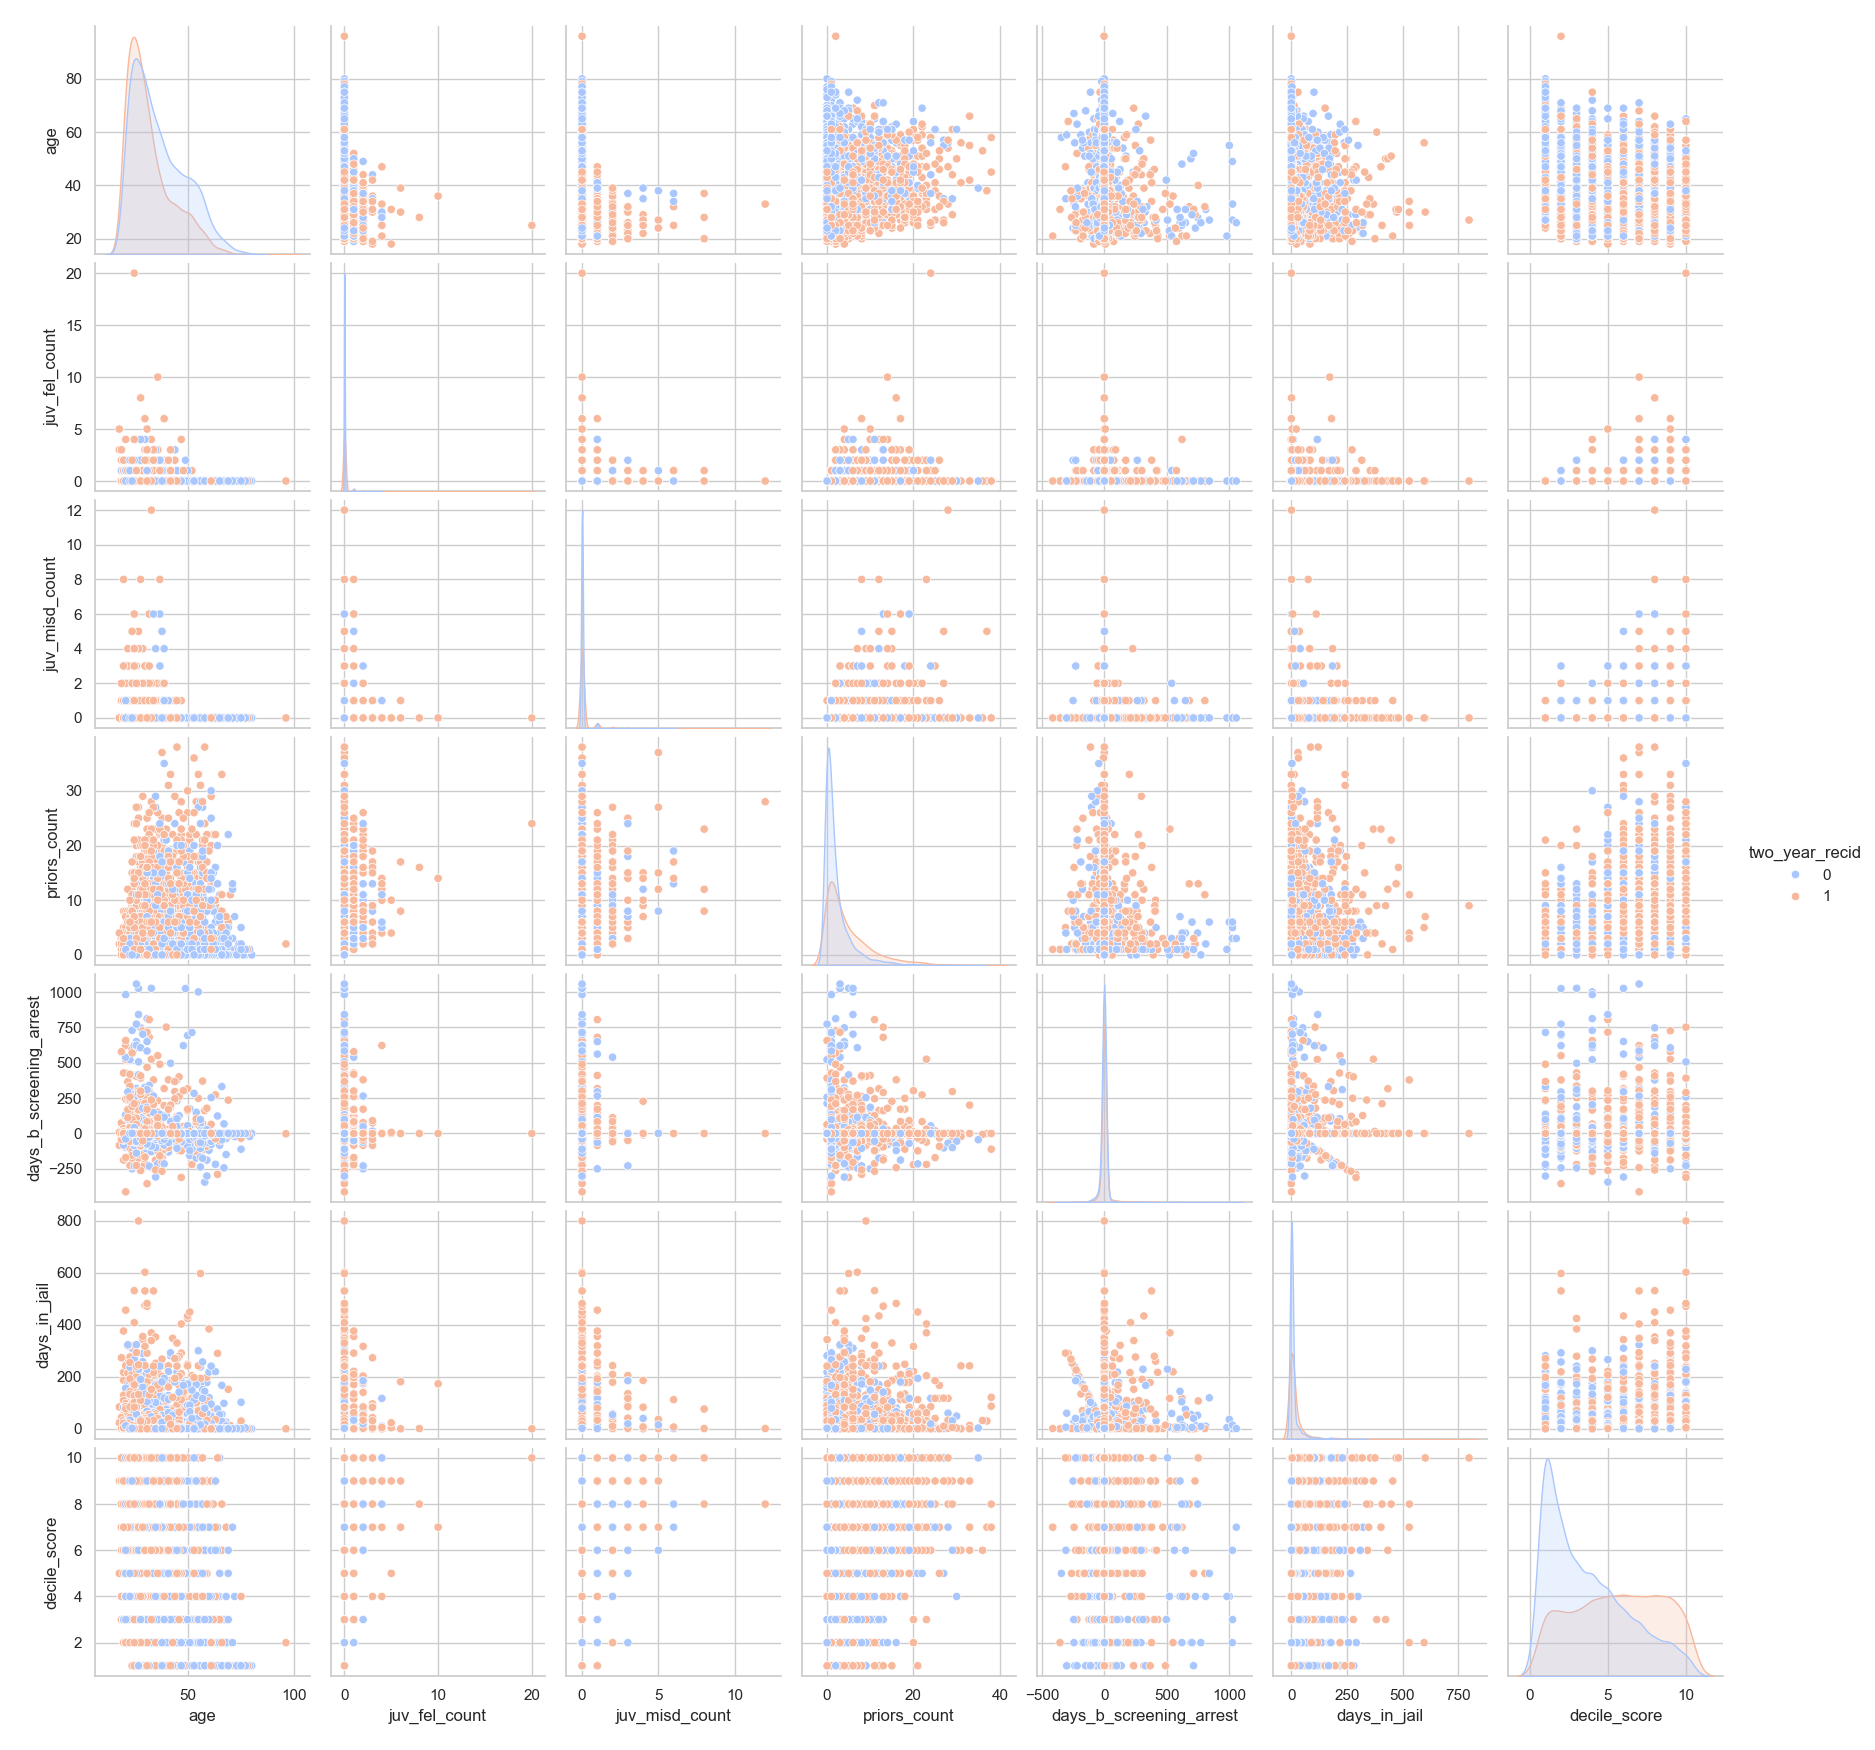
\includegraphics[width=0.7\linewidth]{img/pair_plot}
	\caption{}
	\label{fig:pairplot}
\end{figure}


\begin{itemize}
	\item \textbf{\texttt{age}} vs \textbf{\texttt{priors\_count}}. Younger individuals tend to have fewer prior offences, but the prior count is scattered as age increases, showing that younger offenders tend to continue having problems with the judicial system.
	
	\item \textbf{\texttt{age}} vs \textbf{\texttt{decile\_score}}. Older individuals tend to have lower decile scores. Younger individuals are associated with higher scores.
	
	\item \textbf{\texttt{priors\_count}} vs \textbf{\texttt{decile\_score}}. Positive trend: Higher priors count leads to higher decile scores, suggesting a strong correlation, indicating the tendency for offenders to be viewed as a risk community    
	
	\item The distribution of \textbf{\texttt{decile\_score}}. Two-year recidivists tend to cluster at higher decile scores (6–10 range). Non-recidivists are spread more evenly across scores.        
\end{itemize}



\subsection{Analysis of decile score relationship with race}

The COMPAS dataset has been extensively discussed in recent years regarding the fairness of the scores assigned to individuals, especially considering the race component. Although the tool does not use race as one of the features in decile score prediction, there are concerns that race can be associated indirectly with other features. In this section, we will look at the data from the race point of view to see what patterns we can deduce from the dataset.

As a first step, we create a boxplot to compare the distribution of \textbf{\texttt{decile\_score}} across different racial groups. 

\begin{figure}
	\centering
	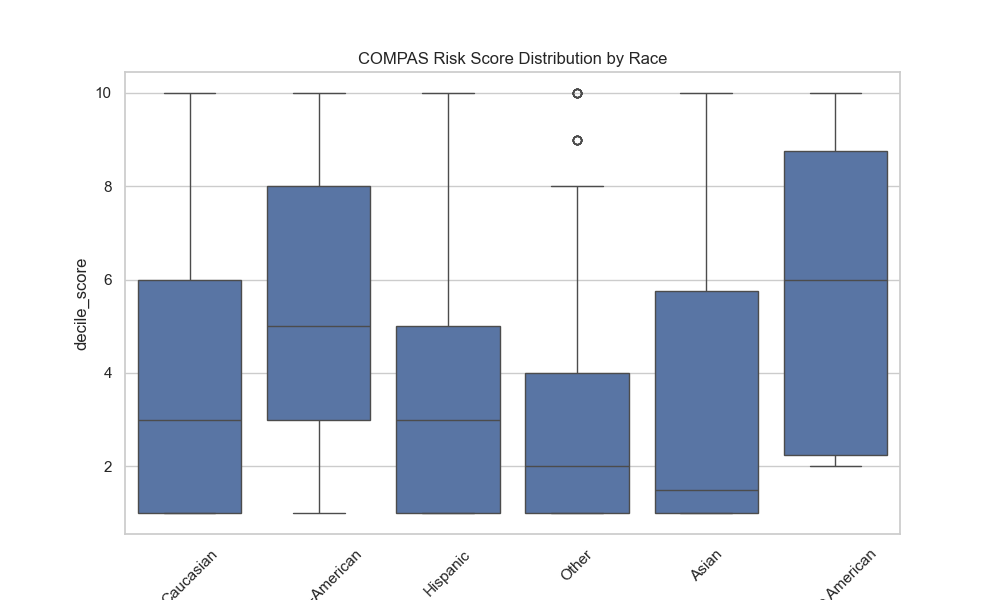
\includegraphics[width=0.7\linewidth]{img/decile_score_by_race_boxplot}
	\caption{}
	\label{fig:decilescorebyraceboxplot}
\end{figure}


From this plot, we notice that African Americans have higher median scores and broader distributions, which suggests a potential bias in the COMPAS scoring system. In addition, Hispanics, Asians, and Other groups scored lower on average, which may indicate differences in the risk assessment process or underlying data inputs.


We then investigated the correlation of \textbf{\texttt{decile\_score}} with \textbf{\texttt{two\_year\_recid}} by race:

\begin{figure}
	\centering
	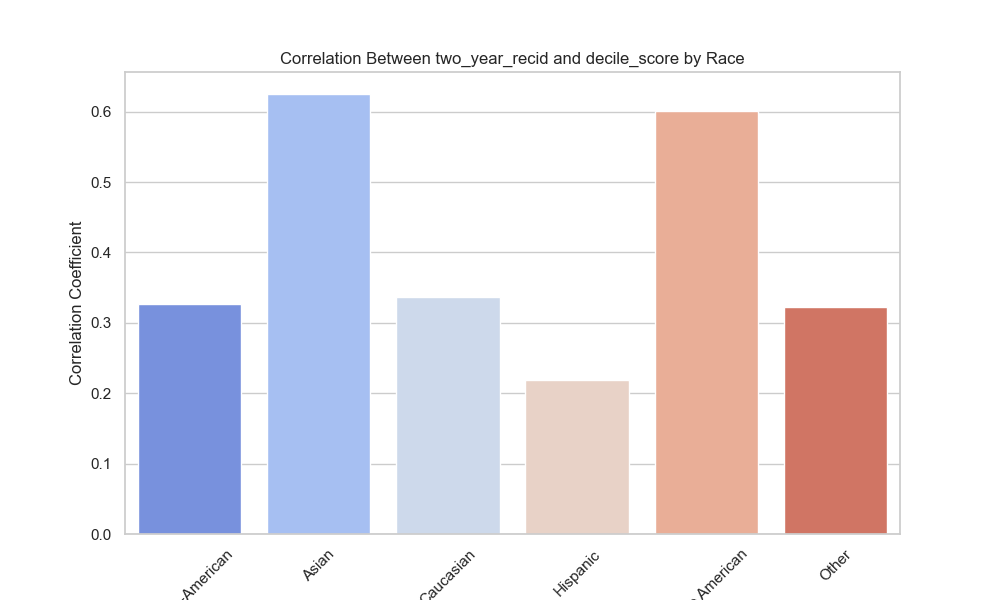
\includegraphics[width=0.9\linewidth]{img/correlation_by_race}
	\caption{}
	\label{fig:correlationbyrace}
\end{figure}

\begin{itemize}
	\item Asians and Native Americans show the highest correlations, indicating that, for these groups, COMPAS scores align more closely with observed recidivism outcomes. However, it is important to remember that these groups comprise a tiny percentage of the population.
	
	\item African-Americans, Caucasians, and Others have moderate correlations, so COMPAS scores are somewhat predictive for these groups but not as strongly as for Asians or Native Americans.
	
	\item The correlation between \textbf{\texttt{two\_year\_recid}} and \textbf{\texttt{decile\_score}} for Hispanics is 0.22, the lowest among the groups, suggesting that for Hispanic individuals, the COMPAS scores are less predictive of actual recidivism outcomes than other racial groups. The low correlation for the Hispanic group is an area of concern because if the COMPAS scores do not accurately predict recidivism for this ethnicity, this could mean that the scoring system may overestimate or underestimate their actual risk, which could lead to misclassification of individuals, leading to potential unfair treatment, for example, harsher parole conditions, sentencing).
\end{itemize}

The distribution of \textbf{\texttt{decile\_score}} for Hispanic individuals was then compared with that of other racial groups using kernel density plots (KDE). 

\begin{figure}
	\centering
	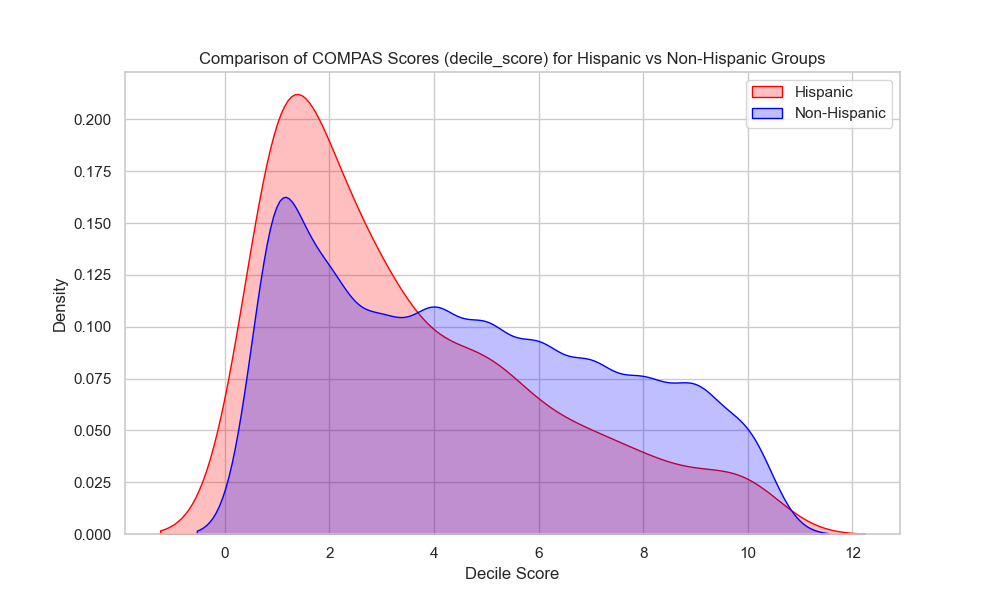
\includegraphics[width=0.7\linewidth]{img/decile_score_by_race_hispanic}
	\caption{}
	\label{fig:decilescorebyracehispanic}
\end{figure}


The plots show that the peak density for Hispanic individuals occurs at a lower score of around 2. In contrast, non-Hispanic individuals have a flatter distribution extending to higher scores, albeit peaking in the same region, suggesting that Hispanic individuals are more likely to receive lower COMPAS scores than non-Hispanic individuals.

One has to note that we have previously seen that Hispanic individuals account for 8.8\% of the population, which is significantly smaller compared to African-American and Caucasian groups.
Although by any means not conclusive, these aspects raise questions about how risk scores are calibrated for underrepresented groups.

\subsubsection{Analysis of the African-American sector}


We created another density plot to compare the distribution of risk scores between African-American individuals and non-African-American individuals.

\begin{figure}
	\centering
	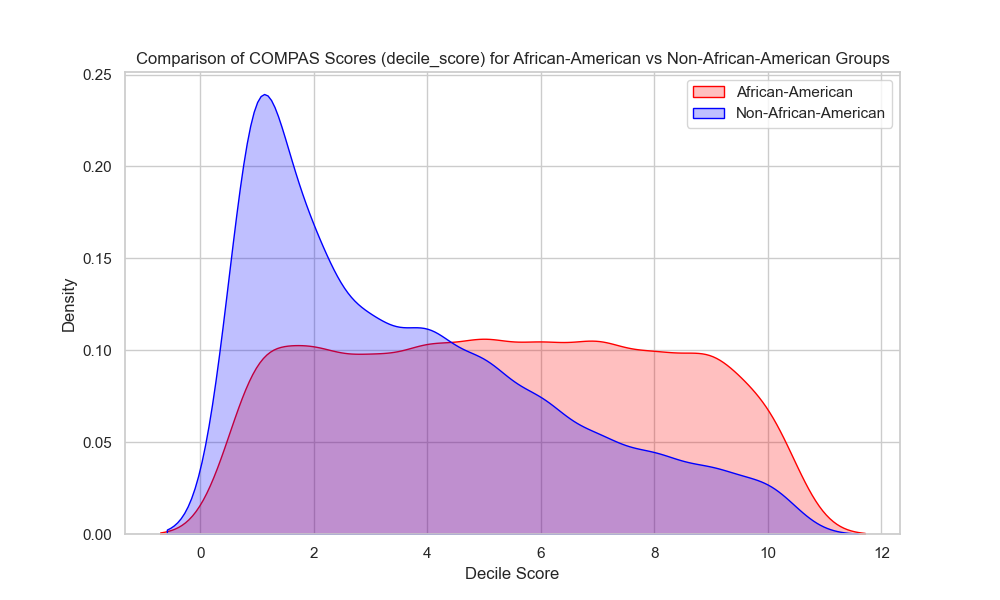
\includegraphics[width=0.7\linewidth]{img/decile_score_by_race_african_american}
	\caption{}
	\label{fig:decilescorebyraceafricanamerican}
\end{figure}


Here, we notice that African Americans are more likely to receive risk scores in the higher decile range, exceeding a value of six, than non-African Americans, suggesting that the COMPAS tool systematically assigns higher risk scores to African Americans. As noticed previously, non-African-American individuals show a strong peak at around a score of 2, with fewer individuals in this group receiving scores in the higher ranges.

This disparity in score distributions raises concerns about potential bias in the COMPAS scoring system. African Americans appear to be disproportionately classified as higher risk, a factor which could impact downstream decisions such as sentencing or parole.

\subsection{Robustness of \textbf{\texttt{decile\_score}}}

As a final analysis, we compare \textbf{\texttt{decile\_score}} with \textbf{\texttt{two\_year\_recid}} to see how many high-risk individuals receded and how many individuals categorised as low-risk did not. This metric is very powerful, as it assesses the validity of the predicted risk metric. Throughout this study, we will also use this test to validate our predicted scores for the machine learning models.


An important decision in this exercise is the selection of the decile score threshold that will dictate that values above it are more likely to recidivate and those below it not. In order to do this, we compared the decile score and two-year record for multiple thresholds. We examined the number of true negatives (the individuals with a decile score lower than the threshold and did not recidivate), true positives (those with a decile score higher or equal than the threshold and did recidivate) and false positives and negatives, and obtained the following results:

\begin{table}[h!] \centering \begin{tabular}{|c|c|c|c|c|} \hline 
		\textbf{Threshold} & \textbf{True Neg} & \textbf{False Pos} & \textbf{True Pos} & \textbf{False Neg} \\ \hline 
		4                               & 2129                   & 1046                    & 964                    & 1632                    \\ \hline 5                               & 2433                   & 742                     & 1243                   & 1353                    \\ \hline 6                               & 2661                   & 514                     & 1529                   & 1067                    \\ \hline 7                               & 2849                   & 326                     & 1805                   & 791                     \\ \hline 8                               & 2979                   & 196                     & 2087                   & 509                     \\ \hline \end{tabular} \caption{Decile Score Threshold Results} \label{tab:decile_scores} \end{table}

We then used these results to calculate the sensitivity, specificity, precision and accuracy:

\begin{table}[h!]
	\centering
	\begin{tabular}{|c|c|c|c|c|}
		\hline
		\textbf{Threshold} & \textbf{Sensitivity} & \textbf{Specificity} & \textbf{Precision} & \textbf{Accuracy} \\ \hline
		4                               & 0.628659             & 0.670551             & 0.60941            & 0.651707          \\ \hline
		5                               & 0.521186             & 0.766299             & 0.645823           & 0.656039          \\ \hline
		6                               & 0.411017             & 0.83811              & 0.674889           & 0.645989          \\ \hline
		7                               & 0.3047               & 0.897323             & 0.708147           & 0.63074           \\ \hline
		8                               & 0.196071             & 0.938268             & 0.721986           & 0.604401          \\ \hline
	\end{tabular}
	\caption{Performance Metrics for Different Decile Score Thresholds}
	\label{tab:performance_metrics}
\end{table}

Following this procedure, a threshold of 5 was decided to provide the best balance of these metrics. With this threshold, the total accuracy and precision are moderate, indicating that while the model performs reasonably well overall, there is room for improvement. We notice a low sensitivity compared to specificity; the model is better at identifying non-recidivists than recidivists.


The metrics for each racial group were then calculated with this threshold.


The Caucasian group has a relatively high specificity but low sensitivity, indicating the COMPAS model more effectively avoids false positives but struggles to identify true positives. 

The African-American group shows higher sensitivity but lower specificity compared to Caucasians. This suggests the model identifies more recidivists among African Americans but at the cost of more false positives.


The Hispanic group has low sensitivity, meaning the model struggles significantly to identify true positives in this group. Precision is also the lowest, indicating a high false-positive rate.


The significant disparity in sensitivity and specificity across racial groups highlights potential fairness issues in the model's predictions. For example, the model disproportionately favours Caucasians and Asians in terms of specificity while penalizing African-Americans with higher false-positive rates.

